%
\section{Introduction}
\label{sec:intro}
\IEEEPARstart{B}{uilding} extraction, which aims to extract rooftop in a large-scale remote sensing image, remains one of the main challenges in the field of remote sensing for several decades. In addition, automatic extraction of building rooftop from aerial and satellite imagery is an important step in many applications, such as: urban planing, automated map making, 3D city modeling, updating geographical dataset and military reconnaissance. It is particularly difficult to extract rooftop from remote sensing images at the pixel level because of the following three reasons: \romannumeral1) Density of the structures in the scene. A rural scene has low density but an urban scene has high density, with a suburban scene in between (medium density).  \romannumeral2) Shape of the structure. Buildings come in many shapes from simple rectangular blocks with flat roof to complex shapes with intricate, multi-based roof structure.  \romannumeral3) Image quality. Images vary in terms of contrast, resolution, and visibility  \cite{IEEEexample:huertas1988detecting}. Some remote sensing patches are shown in Figure 1, which illustrate the difficulties of building extraction task. \par
\begin{figure}
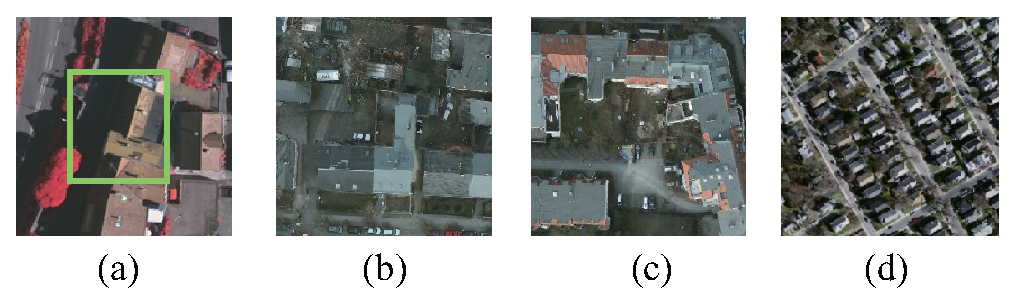
\includegraphics[width=8.7cm]{Figures/challenge.eps}
\caption{Examples of remote sensing patches with different kinds of challenges. (a) Shadow occlusion in green frame. (b) Low inter-class differences. (c) High intra class variance. (d) A lot of tiny buildings close to each other.}
\label{1}
\end{figure}
\setlength{\parindent}{2ex}In the past decades, many investigators made some experimental investigations to extract buildings automatically. In the early days, many knowledge-based methods were put forward by \cite{IEEEexample:huertas1988detecting}, \cite{IEEEexample:noronha2001detection}, \cite{IEEEexample:nosrati2009novel}, \cite{IEEEexample:izadi2012three}, \cite{IEEEexample:wang2015efficient}. Their basic ideas are derived from prior knowledge of buildings, for example buildings are closed polygons made up of some straight lines. Some other methods are based on energy functions, mainly including the variational level set evolution, improved snake model and graph cut \cite{IEEEexample:cote2013automatic}, \cite{IEEEexample:peng2005improved}, \cite{IEEEexample:sirmacek2009urban}.\par
In recent years, with the development of machine learning, some methods via machine learning are gradually penetrating into remote sensing domain. At first, some shallow networks were proposed for multiple object extraction\cite{IEEEexample:mnih2013machine}, \cite{IEEEexample:saito2016multiple}, \cite{IEEEexample:alshehhi2017simultaneous},\cite{IEEEexample:zhao2017contextually}. Afterwards, with the improvement of hardware and computation ability of computer, methods based on deep learning in computer vision are introduced into the field of remote sensing images. Some researchers tried convolutional neural networks for aerial images classification and semantic pixel labelling \cite{IEEEexample:paisitkriangkrai2015effective}, \cite{IEEEexample:liu2017dense}, \cite{IEEEexample:audebert2017deep}, \cite{IEEEexample:kampffmeyer2017urban}, \cite{IEEEexample:he2017multi}.\par
In this work, we propose a modified Convolutional Neural Network (CNN) architecture to extract buildings from satellite imagery by adding fusion sides. Not only the final prediction result obtained by CNN is used, but also the features of other layers are combined. We make full use of low-level appearance information on the basis of high-level semantic information. Numerous experiments on three remote sensing image datasets all obtained fairly good results. After rooftop extracting, the depth map is used to create the point cloud of rooftop. Based on the point cloud, the 3D models are carried out using the method proposed by Zhou\cite{IEEEexample:zhou20112}. Figure 2 illustrates pipeline of our work. Our technical contributions are:\par
 1) A robust CNN which is specially designed for multi-scale building extraction is proposed. It can deal with the problems of different sizes, diverse appearance and mutual occlusion of buildings and etc. The overall accuracy based on HF-FCN exceeds the state-of-art algorithms.\par
 2) Our approach has less computational cost than other methods.\par
 3) A complete system for building extraction and 3D modelling of large-scale urban areas is proposed which makes the process of building extraction efficiently. And the building extraction part is a end-to-end network that does not need any post processing.
\begin{center}
\begin{figure}
\includegraphics[width=8.7cm]{Figures/pipeline.eps}
\caption{An overview of proposed urban 3D modelling framework. The inputs of our system are multi-channel images. Semantic segmentation that extracts building areas from aerial images is the first step. After it, we generate the point cloud according to the DSM. Based on the point cloud, the 3D reconstruction is implemented.}
\label{2}
\end{figure}
\end{center}
\subsection{Paper Organization}
\setlength{\parindent}{2ex}The remainder of this paper is organized as follows. Section \uppercase\expandafter{\romannumeral2} summed up the related past works. In Section \uppercase\expandafter{\romannumeral3} we introduce the architecture of our network and show the training steps of our HF-FCN. And in Section \uppercase\expandafter{\romannumeral4}, a brief description of the dataset used for our task is provided. HF-FCN training strategies, details and its evaluation metrics are described. In Section \uppercase\expandafter{\romannumeral5} we present the experimental results and the results of 3D modeling. Finally, the conclusion and discussion are discussed in Section\uppercase\expandafter{\romannumeral6}.
